%Demonstra como foi realizado o trabalho
%• Pesquisas bibliográficas: sempre com as referências
%• Modelagem
%• Sistema gerado
%• Testes de desempenho/avaliação
\chapter{Fundamentação Teórica}
\label{cap:methods}
\noindent

Aprendizado de máquina é um ramo da inteligência artificial na Ciência da Computação em que se faz uso de dados para o desenvolvimento de um algoritmo por meio de etapas de treinamento. Mais especificamente no aprendizado supervisionado, estuda-se um conjunto de dados rotulados na fase de treinamento para que o algoritmo treinado possa prever um rótulo de um dado inédito baseando-se nos padrões já estudados. Para a classificação de textos em assuntos, o aprendizado supervisionado é o mais utilizado, de maneira que os rótulos correspondem aos próprios assuntos dos textos a serem utilizados no treinamento.

Contudo, uma dificuldade ao se trabalhar com um texto é o uso de uma representação computacional que seja facilmente interpretável pelos algoritmos de aprendizado de máquina. Por isso, são utilizadas representações específicas para esses algoritmos como Bag of Words e Word Embeddings que serão descritos nas seções a seguir. Posteriormente, pode-se aplicar algoritmos como, por exemplo, redes neurais que também serão descritas nas seções seguintes.

\section{Bag of Words}
%https://www3.nd.edu/~dchiang/teaching/nlp/2015/notes/chapter1v2.pdf
%https://towardsdatascience.com/machine-learning-nlp-text-classification-using-scikit-learn-python-and-nltk-c52b92a7c73a

Bag of words não se trata de um modelo de classificação por completo, mas sim de uma estratégia de representação do texto em que a sequência de palavras é desconsiderada. Dessa maneira, o texto é simplificado para uma lista de palavras distintas e a respectiva contagem de ocorrência de cada uma delas. A principal vantagem dessa estratégia é a sua simplicidade de representação computacional, sendo atrativa para a aplicação direta de algoritmos de aprendizado de máquina.

Contudo, para se obter uma melhor eficiência dessa estratégia, pode ser necessário aplicar outras técnicas que mitiguem a perda de informação causada pelo \textit{bag of words}. Uma dessas técnicas é a remoção de palavras de parada (stop words), pois essas palavras são utilizadas apenas para a conexão de ideias em uma frase como preposições, artigos e conjunções e não contribuem como fonte de informação no texto. Além disso, as palavras vazias ocorrem com alta frequência e possuem destaque ilusório na representação colapsada do bag of words. Outra técnica que também pode ser empregada é a lematização (\textit{stemming}) que corresponde a remoção dos sufixos das palavras, pois estes fazem com que palavras que deveriam ser sinônimas na representação \textit{bag of words} sejam contabilizadas separadamente. Ao remover os sufixos como gênero, tempo e número, palavras que acrescentam a mesma informação ao texto terão suas respectivas contagens somadas em uma única palavra sem os sufixos. A figura \ref{fig:nl_ex} mostra um exemplo dessas etapas de pré-processamento.

\begin{figure}[!ht]
	\centering
	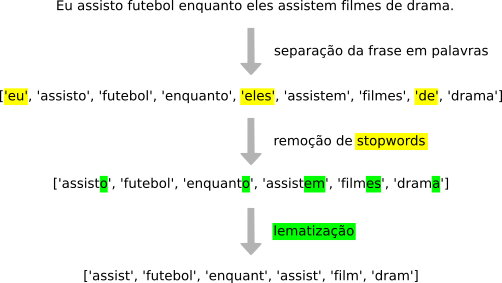
\includegraphics[width=1\textwidth]{figures/nltp_example.png}
	\caption{Etapas do processamento de linguagem natural}
	\label{fig:nl_ex}
\end{figure}

Após todas essas técnicas, pode-se extrair ainda a representação TF-IDF (\textit{term frequency-inverse document frequency}), \cite{InformationRetrievalBookChapter6}, de cada amostra de um conjunto de textos, trata-se de uma medida estatística para normalizar o peso das palavras. Nesse indicador, a relevância de uma palavra em determinado contexto é representada pelo número de vezes que a palavra nesse contexto dividido pelo número de vezes que ela aparece em todos os documentos que fazem parte do \textit{corpus} analisado. A figura \ref{fig:bow_ex} mostra um exemplo da representação de dois documentos conforme a modelagem \textit{bag of words}.

\begin{figure}[!ht]
	\centering
	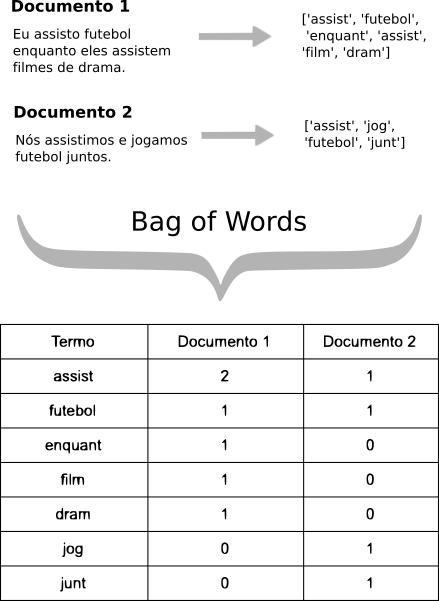
\includegraphics[width=0.7\textwidth]{figures/bag_of_words_example.png}
	\caption{Exemplo de representação \textit{bag of words}}
	\label{fig:bow_ex}
\end{figure}

\section{Word Embeddings}

Word embedding é a representação de palavras de um vocabulário em um espaço n-dimensional de números reais. Isso permite que palavras que são usadas de maneira similar tenham representações similares, de maneira a capturar o significado de cada palavra de acordo com a sua posição no espaço n-dimensional. Cada palavra é mapeada a um vetor e os valores desse vetor são obtidos a partir de um treinamentos que, em geral, envolvem redes neurais como o skip-gram utilizado na implementação word2vec, \cite{DBLP:journals/corr/MikolovSCCD13}.

\section{Redes Neurais Artificiais}

Redes Neurais são uma classe de funções em que a sua formulação matemática foi vagamente inspirada em estruturas biológicas do cérebro. Na analogia biológica dessa formulação, essas funções podem ser representadas no formato de um grafo em que as estruturas básicas são chamadas neurônios.

\begin{figure}[!ht]
	\centering
	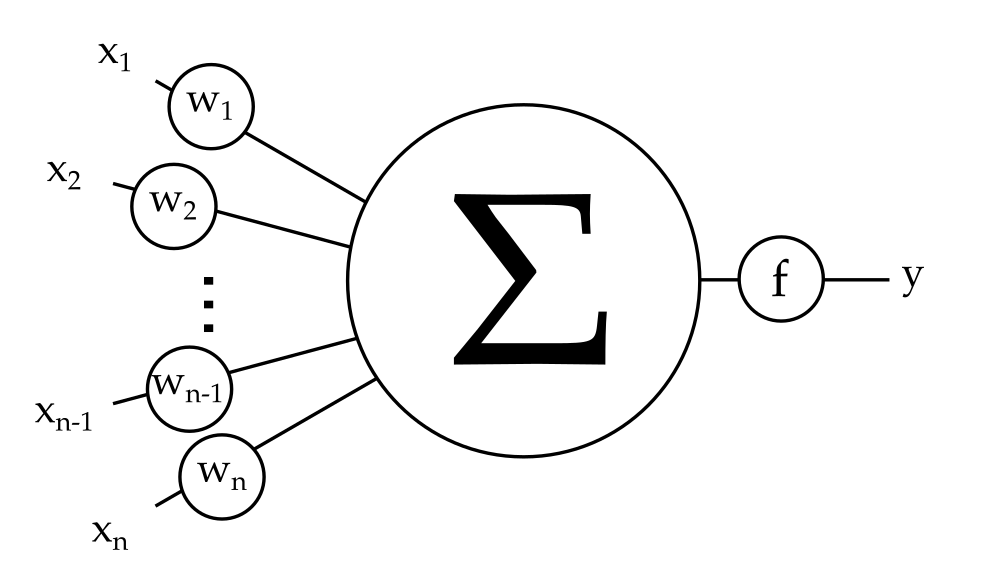
\includegraphics[width=0.6\textwidth]{figures/neuron.png}
	\caption{Neurônio artificial}
	\label{fig:neuron}
\end{figure}

Conforme a figura \ref{fig:neuron}, um neurônio artificial é uma função $y:\mathbb R^n \rightarrow \mathbb R$ com entrada $\vec x = <x_1,x_2,x_3,\dots,x_n>$ e saída $y = f(\sum\limits_{i=1}^n x_iw_i)$, em que $f$ é a chamada função de ativação, correspondendo tradicionalmente a função sigmoid, mas atualmente a função mais utilizada é a relu ($f(x) = max(0, x)$).

Os parâmetros que definem a arquitetura de uma rede neural tradicional dentro do conjunto da classe de funções são chamados hiperparâmetros. Esses parâmetros definem a quantidade de neurônios e as conexões entre eles que são tradicionalmente organizadas segundo camadas totalmente conectadas.

Uma característica que torna as redes neurais interessantes é o fato de elas atenderem ao Teorema da aproximação universal segundo \cite{HORNIK1991251}. Contudo, o que as tornam realmente especiais no contexto de aprendizado de máquinas é a maneira com que são encontrados os parâmetros para a aproximação de funções. Diferentemente da aproximação de funções diferenciáveis pelo teorema de Taylor por exemplo, existem heurísticas que permitem encontrar os parâmetros de uma rede neural para a aproximação da função a partir de amostras pontuais, i.e., dados, sem que seja necessário o conhecimento da função original como formulado no teorema de Taylor.

Dessa maneira, além dos hiperparâmetros, há as duas seguintes categorias de parâmetros em uma rede neural: parâmetros treináveis que são escolhidos a partir de procedimentos de treinamento envolvendo dados para a aproximação de funções; parâmetros de entrada que correspondem aos da função que se deseja aproximar. Uma vez encontrados parâmetros treináveis para uma aproximação satisfatória, estes são fixados e utilizam-se os parâmetros de entrada para realizar previsões nas situações de interesse.

Uma vez que a definição de parâmetros treináveis já foi realizada, pode-se retomar a análise das heurísticas que permitem determiná-los. Esse processo consiste em um algoritmo iterativo que minimiza uma função de custo baseada na comparação entre a saída da rede neural atual com dados de treinamento e os respectivos valores reais. Esse processo é chamado método do gradiente e, conforme o próprio nome diz, exige o cálculo do gradiente da função de custo em relação aos parâmetros treináveis e é viabilizado pelo algoritmo backpropagation por \cite{Rumelhart1986}. Atualmente, são utilizadas diversas técnicas para a otimização do método do gradiente \cite{DBLP:journals/corr/Ruder16}, envolvendo desde variações na forma como as variáveis são atualizadas no processo iterativo quanto como inicializar os parâmetros treináveis ou execuções em mini-batches.

\subsection{Redes Neurais Convolucionais}
Redes neurais convolucionais consistem em uma variação da arquitetura de redes neurais tradicionais em que parâmetros treináveis podem ser reutilizados em diferentes operações durante o cálculo de feedforward de uma rede neural. Isso permite o reconhecimento de um mesmo padrão em distintos subconjuntos dos dados de entrada, tornando esse tipo de arquitetura ideal para reconhecimento de objetos em imagens conforme originalmente descrito por \cite{LeCun1999}. Contudo, uma variação unidimensional da rede neural convolucional também pode ser útil no reconhecimento de padrões em textos com o auxílio de word embeddings.

\subsection{Redes Neurais Recorrentes}

Conforme ilustrado por \cite{ColahLSTM}, redes neurais recursivas são uma extensão das redes neurais tradicionais que visam permitir a representação de um estado de memória no processo de feedforward da rede. Isso é especialmente útil quando os dados de entrada dependem de uma sequência para possuírem coerência, como ocorre no caso de um texto. A extração máxima de informação de um texto só ocorre quando se leva em consideração a sequência das palavra, o que não é tratado no método bag of words por exemplo.

A representação de estado de memória em uma rede neural é viabilizada por meio de uma célula, i.e., um conjunto de neurônios com operações que são aplicadas uma vez para cada elemento da sequência de um dado de entrada. Dessa maneira, além de haver um compartilhamento de parâmetros treináveis como nas redes neurais convolucionais, também há um estado armazenado nos neurônios da célula que são realimentados a essa mesma célula ao executar as operações envolvendo o elemento seguinte da sequência, o que dá origem ao nome recorrente.
